\chapter{理论力学}
\section{广义坐标;拉格朗日量}
高中里我们学的是牛顿力学,但是世界上除了牛顿力学,还有别的力学体系,拉格朗日力学是其中常用的一种。要学习拉格朗日力学,首先要忘掉牛顿力学的世界观。假设我们不知道什么叫力,什么叫能量,什么叫速度,也不知道牛顿定律之类的东西。

我们要研究一个力学系统,就要用一些坐标来描述它。比如平面上的一个点可以用直角坐标$x$、$y$来描述,也可以用极坐标$r$、$\theta$来描述。如图\ref{fig-double-pend},平面内的双摆可以用坐标$\theta$、$\phi$来描述。
\begin{figure}[htb]
\centering
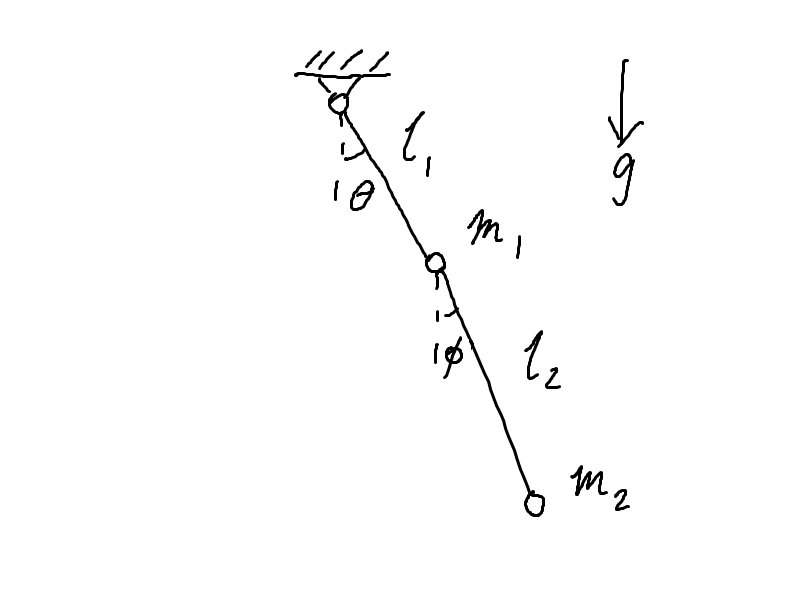
\includegraphics[scale=0.5]{fig/double-pend}
\caption{双摆}
\label{fig-double-pend}
\end{figure}

这里的坐标一般是位置或者角度,也可以是电量、温度等等。牛顿力学中的速度有时候也可以作为这里的坐标,但是现在先不考虑这件事情。

坐标对时间的导数叫作速度。出于习惯,用$\dot x$表示$\frac{\opd x}{\opd t}$,$\dot x^2$表示$(\frac{\opd x}{\opd t})^2$,而不是$\frac{\opd x^2}{\opd t}$,$\ddot x$表示$\frac{\opd^2 x}{\opd t^2}$。

拉格朗日力学的第一个基本假设是:每个力学系统都有一个“拉格朗日量”。比如一个小球在竖直平面内,用坐标$x$、$y$描述它的位置,考虑沿$-y$方向的重力场,那么它的拉格朗日量是
\begin{equation*}
L=\frac{1}{2}m(\dot x^2+\dot y^2)-m g y
\end{equation*}

诶这个东西看起来很像牛顿力学中的能量,但是仔细看会发现势能的正负号反了一下。拉格朗日量一般是坐标和速度的函数,而不会出现坐标的二阶或更高阶导数,而坐标和速度又是时间的函数。如果出现随时间变化的电场之类的环境条件,那么拉格朗日量本身还是时间的函数,但是现在也不考虑这件事情。

这个基本假设并不能告诉我们拉格朗日量是什么,就像从牛顿第二定律不能推出万有引力定律$F=\frac{G M m}{r^2}$一样。它们需要用其他方法推导出来,并且经过实验验证。比如自由粒子的拉格朗日量为$\frac{1}{2}m \mathbf{v}^2$,有质量的粒子在$-y$方向的重力场里要增加一项$-m g y$,带电粒子在电场中要增加一项$-q \phi$,在磁场中要增加一项$q \mathbf{v} \cdot \mathbf{A}$(这个看不懂可以先不管)。

图\ref{fig-double-pend}中双摆的拉格朗日量是
\begin{equation*}
L=\frac{1}{2}m_1 l_1^2 \dot \theta^2+\frac{1}{2}m_2 l_2^2 \dot \phi^2+m_1 g l_1 \cos \theta+m_2 g (l_1 \cos \theta+l_2 \cos \phi)
\end{equation*}

这已经是很复杂的拉格朗日量了,接下来要遇到的东西没有这么复杂。
\section{变分;拉格朗日方程}
把拉格朗日量写出来之后,可以用它来算出物体的运动情况。简单起见,假设系统只有一个坐标$q$,速度为$\dot q$。如果已知物体在时间$t_1$的坐标为$q_1$,时间$t_2$的坐标为$q_2$,但是不知道$t_1$和$t_2$之间的坐标$q(t)$。现在定义一个\emph{作用量}
\begin{equation*}
S=\int_{t_1}^{t_2} L(q(t),\dot q(t)) \opd t
\end{equation*}

它表示物体在$t_1$和$t_2$之间的运动。物体可以做我们熟悉的斜抛之类的运动,也可以做各种奇怪的运动,如图\ref{fig-strange-move},只要保证$q(t_1)=q_1$,$q(t_2)=q_2$这两个边界条件就行。
\begin{figure}[htb]
\centering
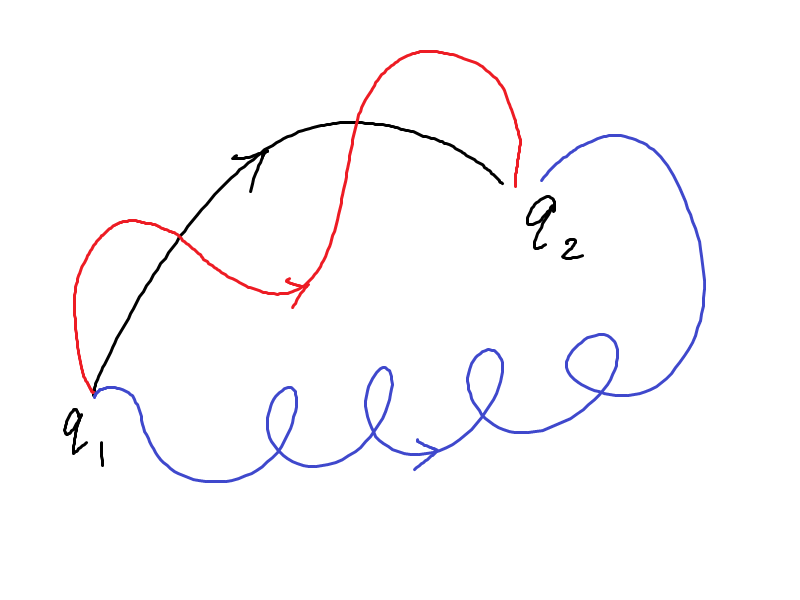
\includegraphics[scale=0.5]{fig/strange-move}
\caption{奇怪的运动}
\label{fig-strange-move}
\end{figure}

现在是拉格朗日力学的第二个基本假设:在这些奇怪的运动当中,真正的运动算出来的$S$是一个极小值。用数学语言来描述,就是
\begin{equation*}
\opvar S=0
\end{equation*}

这就是传说中的\emph{变分原理}!!是不是觉得拉格朗日的脑洞比牛顿还大?

(前方高能,看不懂可以先跳过)

$\opvar$表示变分,它的作用和求导差不多,而且目前我们认为它和积分、求导可以交换顺序。
\begin{align*}
\opvar S&=\opvar \int_{t_1}^{t_2} L(q(t),\dot q(t)) \opd t \\
&=\int_{t_1}^{t_2} \opvar L(q(t),\dot q(t)) \opd t \\
&=\int_{t_1}^{t_2}(\frac{\partial L}{\partial q} \opvar q+\frac{\partial L}{\partial \dot q} \opvar \dot q)\opd t \\
&=\int_{t_1}^{t_2}\frac{\partial L}{\partial q} \opvar q \opd t+\int_{t_1}^{t_2}\frac{\partial L}{\partial \dot q} (\opvar \frac{\opd q}{\opd t}) \opd t \\
&=\int_{t_1}^{t_2}\frac{\partial L}{\partial q} \opvar q \opd t+\int_{t_1}^{t_2}\frac{\partial L}{\partial \dot q} (\opdt \opvar q) \opd t
\end{align*}

对后面一项用分部积分:
\begin{align*}
\opdt(\frac{\partial L}{\partial \dot q} \opvar q)&=\opdt(\frac{\partial L}{\partial \dot q}) \opvar q+\frac{\partial L}{\partial \dot q} (\opdt \opvar q) \\
\frac{\partial L}{\partial \dot q} (\opdt \opvar q)&=\opdt(\frac{\partial L}{\partial \dot q} \opvar q)-\opdt(\frac{\partial L}{\partial \dot q}) \opvar q \\
\int_{t_1}^{t_2}\frac{\partial L}{\partial \dot q} (\opdt \opvar q) \opd t&=\int_{t_1}^{t_2} \opdt(\frac{\partial L}{\partial \dot q} \opvar q) \opd t-\int_{t_1}^{t_2}\opdt(\frac{\partial L}{\partial \dot q}) \opvar q \opd t\\
&=\left. \frac{\partial L}{\partial \dot q} \opvar q \right|_{t_1}^{t_2}-\int_{t_1}^{t_2}\opdt(\frac{\partial L}{\partial \dot q}) \opvar q \opd t
\end{align*}

$t_1$和$t_2$时的坐标是确定的,所以$\opvar q=0$,只剩下后面一项。继续算$\opvar S$:
\begin{align*}
\opvar S&=\int_{t_1}^{t_2}\frac{\partial L}{\partial q} \opvar q \opd t-\int_{t_1}^{t_2}\opdt(\frac{\partial L}{\partial \dot q}) \opvar q \opd t \\
&=\int_{t_1}^{t_2}(\frac{\partial L}{\partial q}-\opdt\frac{\partial L}{\partial \dot q}) \opvar q \opd t
\end{align*}

(高能部分结束)

要让$\opvar S=0$,那么$\frac{\partial L}{\partial q}-\opdt \frac{\partial L}{\partial \dot q}=0$。这就是拉格朗日力学中的运动方程。

有多个坐标的时候的推导也是类似的。比如有两个坐标$x$和$y$,那么就有两个方程$\frac{\partial L}{\partial x}-\opdt \frac{\partial L}{\partial \dot x}=0$,$\frac{\partial L}{\partial y}-\opdt \frac{\partial L}{\partial \dot y}=0$。

用掉下来的小球的例子试一试:$L=\frac{1}{2}m(\dot x^2+\dot y^2)-m g y$,$\frac{\partial L}{\partial y}=-m g$,$\frac{\partial L}{\partial \dot y}=m \dot y$,$\opdt \frac{\partial L}{\partial \dot y}=m \ddot y$,代入运动方程得到$-m g-m \ddot y=0$,也就是说$\ddot y=-g$,跟我们的常识一样。

(注意:对$q$求导时$\dot q$当作常数,对$\dot q$求导时$q$当作常数)

严格来说,变分为零只表示作用量达到极值或者稳定值,而不一定是极小值,跟导数的道理一样。但是物理问题里遇到的一般都是极小值,所以“作用量取极小值”成了一个约定俗成的说法。

在力学范围内,拉格朗日量是坐标和速度的函数,所以只要知道系统在某个时刻的坐标和速度,就能算出它在从前和将来任何时候的坐标、速度、加速度、能量等情况,这就是牛顿时代决定论的思想。但是热学范围内出现了一些不能这样描述,或者说不可逆的过程,比如粘滞阻力或者铁的磁化,怎样用力学原理来解释这些现象是至今还在研究的问题。

变分原理在物理学的其他领域也会出现,比如光学里的光程最短原理,只要定义作用量为$S=\int_{\mathbf{r}_1}^{\mathbf{r}_2} n(\mathbf{r}) \opd \mathbf{r}$,$\mathbf{r}$表示空间中的位置,$n(\mathbf{r})$表示这个位置的折射率,那么$\opvar S=0$就能给出光走的路线。
\section{对称性与守恒量;动量;能量}
还是看掉下来的小球的例子:$L=\frac{1}{2}m(\dot x^2+\dot y^2)-m g y$。如果对$x$坐标列运动方程会怎么样呢?拉格朗日量不含$x$,所以$\frac{\partial L}{\partial x}=0$,$x$坐标的运动方程就是$\ddot x=0$。

现在定义$\frac{\partial L}{\partial \dot q}$叫作坐标$q$对应的动量$p_q$。在上面的例子中,$x$坐标对应的动量就是$m \dot x$,跟牛顿力学一样。因为拉格朗日量不含$x$,所以$\opdt p_x=0$,这个动量是守恒的。

拉格朗日量不含$x$,也可以说系统具有空间平移对称性。所以就有了这样一句话:空间的平移对称性导致动量守恒。

刚才的数学推导看起来很厉害,现在用人话再解释一遍。如果一个小球在一片平地上跑,它向前跑了一段,前面还是一片平地,也就是说系统平移之后和原来一样,因此我们说系统具有平移对称性。在这样的系统中,小球没有理由改变它的动量,动量是守恒的。

(系统平移之后,小球的位置(或者说坐标)就变了,但是拉格朗日量的表达式不变,所以我们认为系统和原来一样。关于对称性的严格定义以后应该会单独讲)

如果小球向前跑,撞到一面墙弹回来,它的动量就不守恒了。这个系统没有平移对称性,如果把系统平移一下,墙的位置就变了。也就是说,平移对称性的破缺导致动量守恒的破缺。如果小球在斜坡上跑,它会越跑越快。虽然向前跑一段之后,斜坡的斜率还是和原来一样,但是高度变了(或者说重力势能与水平坐标的关系变了),所以这个系统没有平移对称性,动量也就不守恒。

如果拉格朗日量不含时间$t$,又会发生什么呢?
\begin{align*}
\opdt L&=\frac{\partial L}{\partial q} \frac{\opd q}{\opd t}+\frac{\partial L}{\partial \dot q} \frac{\opd \dot q}{\opd t} \\
&=(\opdt \frac{\partial L}{\partial \dot q}) \frac{\opd q}{\opd t}+\frac{\partial L}{\partial \dot q} \frac{\opd \dot q}{\opd t} \\
&=\opdt(\frac{\partial L}{\partial \dot q} \dot q) \\
&=\opdt(p \dot q)
\end{align*}

(注意:因为拉格朗日量不含$t$,所以不会出现$\frac{\partial L}{\partial t}$)

移项得到$\opdt(p \dot q-L)=0$,所以可以定义$p \dot q-L$叫作能量$E$。如果有多个坐标,那么能量$E=\sum_i p_i \dot q_i-L$。用掉下来的小球算一下会发现这个能量和牛顿力学里的能量其实是一样的。

也就是说,时间的平移对称性导致能量守恒。比如一个单摆挂在那里摆动,过了一段时间,系统还是和原来一样,所以单摆的能量是守恒的。如果过了一段时间,突然让单摆带电,并且在空间中加一个电场,这个系统就没有时间平移对称性,能量也就不守恒了。这里没有考虑摩擦力、空气阻力之类的,事实上这些力在拉格朗日力学当中不能用简单的方法处理,但是我们认为它们会破坏系统的时间平移对称性。

如果坐标是角度,那么对应的动量就是牛顿力学中的角动量。但是拉格朗日力学对角动量有另外的定义,空间的旋转对称性导致角动量守恒,这里先不讲了。对称与守恒在物理学当中非常重要,以后我们还会遇到更奇怪的对称性和它对应的守恒量。

总而言之,拉格朗日力学是一种与牛顿的基础完全不同的力学方法,它的优点在于不用做受力分析,而且容易处理守恒量。工程师用电脑计算桥梁之类的复杂结构用的就是这种方法,因为电脑很难做受力分析,但是适合算各种偏导数。现代的粒子物理当中,两个粒子之间“力”的概念也很难说清楚,所以也要用这种方法处理。如果我们发现了新的粒子,想办法确定它的拉格朗日量是一件很重要的事情。
\section{虚功原理}
拉格朗日力学只是扩大一下大家的眼界,现在我们回到牛顿力学。

一个掉下来的小球,它的能量是$E=\frac{1}{2}m(\dot x^2+\dot y^2)+m g y$。把能量对时间求导:
\begin{align*}
\opdt E&=m(\dot x \ddot x+\dot y \ddot y)+m g \dot y \\
&=m \ddot x \dot x+(m \ddot y+m g) \dot y
\end{align*}

又因为能量守恒,$\opdt E=0$。不管小球的速度是多少,这个式子都是成立的,而且$\dot x$和$\dot y$是无关的,所以它们前面的系数都要为$0$,于是我们得到了$\ddot x=0$,$\ddot y=-g$。

(这样推导应该比拉格朗日量之类的好理解一点,但是如果承认拉格朗日量就是动能减势能,通过一些分部积分,这种方法和拉格朗日力学的基本假设是可以互相推导的。为什么说$\dot x$和$\dot y$是无关的呢?这个待会再讲)

很多书都在静力学中用虚功原理,事实上在动力学中也是可以用的。
\begin{figure}[htb]
\centering
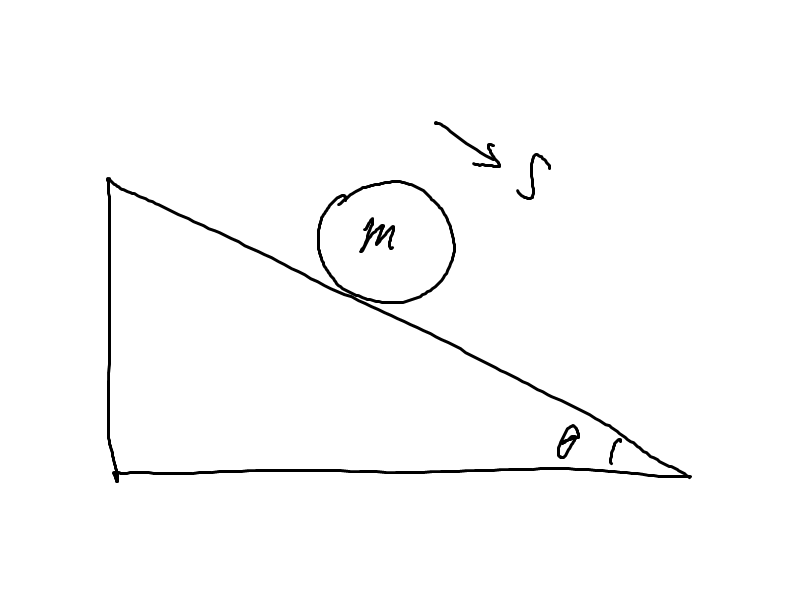
\includegraphics[scale=0.5]{fig/slope-ball}
\caption{卧槽,一个球滚下来了!}
\label{fig-slope-ball}
\end{figure}

现在来看一个复杂一点的例子:如图\ref{fig-slope-ball},一个固定粗糙斜面倾角为$\theta$,一个质量为$m$的均匀空心球壳无滑动地滚下来,设沿斜面的位移为$s$,球心的速度就是$\dot s$,但是考虑转动之后,它的动能不是$\frac{1}{2} m \dot s^2$,而是$\frac{5}{6} m \dot s^2$,现在要算它滚下来的加速度。正常的自招书上会用受力分析啊转动定律啊速度关联之类的来算,但是现在我们用虚功原理。

先写出系统的能量:$E=\frac{5}{6} m \dot s^2+m g s \sin \theta$,然后对时间求导:$(\frac{5}{3} m \ddot s+m g \sin \theta) \dot s=0$,所以$\ddot s=-\frac{3}{5} g \sin \theta$。

【练习】如果是均匀实心球,那么动能是$\frac{7}{10} m \dot s^2$。求它的加速度,然后算出速度和位移关于$t$的函数,并且验证能量确实是守恒的。
\section{约束;自由度}
再增加一点难度:假设斜面是会动的,质量为$M$。但是斜面是光滑的,这样球就不会转动,它的动能是$\frac{1}{2} m v^2$,否则太难了。
\begin{figure}[htb]
\centering
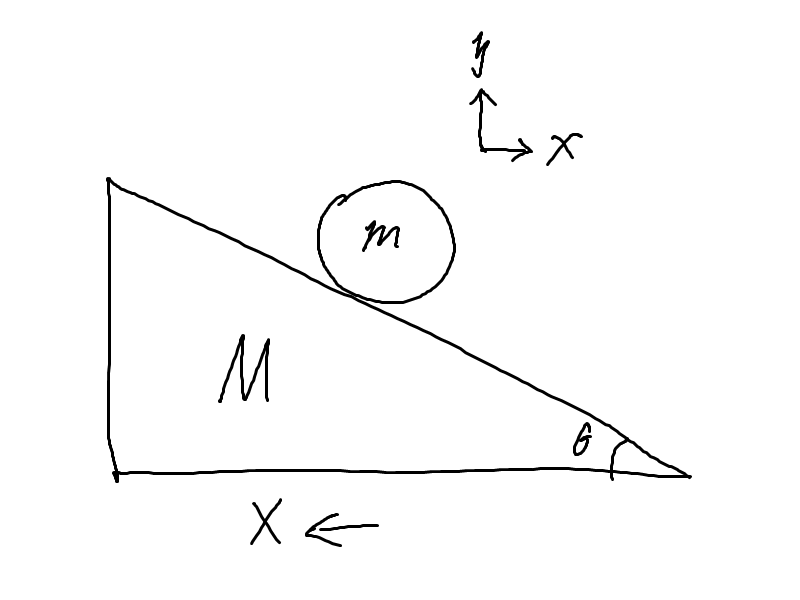
\includegraphics[scale=0.5]{fig/slope-ball-2}
\caption{卧槽,球和斜面都在动!}
\label{fig-slope-ball-2}
\end{figure}

现在把坐标设为$s$就不太方便了,如图\ref{fig-slope-ball-2},把$M$向左的位移设为$X$,把$m$的位移设为$x$和$y$。系统的能量是$E=\frac{1}{2} M \dot X^2+\frac{1}{2} m (\dot x^2+\dot y^2)+m g y$。

但是!坐标$X$、$x$和$y$并不是无关的。小球必须在斜面上,所以有一个约束条件$y=-(X+x) \tan \theta$。这个约束条件还可以求导得到$\dot y=-(\dot X+\dot x) \tan \theta$。

在$E$里把$y$消掉,得到$E=\frac{1}{2} M \dot X^2+\frac{1}{2} m (\dot x^2+(\dot X+\dot x)^2 \tan^2 \theta)-m g (X+x) \tan \theta$。

现在$X$和$x$是无关的,把能量对时间求导,经过各种化简得到$((M+m \tan^2 \theta) \ddot X+m \tan^2 \theta \ddot x-m g \tan \theta)\dot X+(m \tan^2 \theta \ddot X+m (1+\tan^2 \theta) \ddot x-m g \tan \theta)\dot x=0$。

要求$\dot X$和$\dot x$的系数都为零,解得$\ddot X=\frac{m \tan \theta}{M (1+\tan^2 \theta)+m \tan^2 \theta} g$,$\ddot x=\frac{M \tan \theta}{M (1+\tan^2 \theta)+m \tan^2 \theta} g$。代入$y$的式子得$\ddot y=-\frac{(M+m) \tan^2 \theta}{M (1+\tan^2 \theta)+m \tan^2 \theta} g$。

把题目做完之后,考虑几个特殊情况:如果$M \gg m$,那么跟斜面不动的时候一样,$\ddot y=-g \tan^2 \theta$;如果$M \ll m$,那么小球几乎是竖直掉下来,$\ddot y=-g$。

这个系统有$3$个坐标,$1$个约束,所以有$3-1=2$个独立的坐标,或者说有$2$个自由度。如果把斜面左右移动设为一个坐标,小球沿着斜面上下移动设为另一个坐标,那么就没有约束条件了,系统仍然有$2$个自由度。同一个系统,不管选择什么坐标,自由度的数量总是一样的。

比如三维空间中的质点有$3$个自由度,不管你用直角坐标、柱坐标还是球坐标。如果是一个会转的小球,要确定它的方向,就多了$3$个转动自由度,总共$6$个自由度。

(严格来说这里只考虑完整约束,也就是斜面与小球的位置关系,而与它们的速度无关。非完整约束这里先不讲)

我们发现$M \dot X=m \dot x$(注意$X$和$x$设的正方向),也就是水平方向动量守恒。动量守恒并不是一个约束条件,而且一般情况下能量守恒和动量守恒是不能互推的。但是如果把动量守恒当作一个已知条件,上面的计算可以简化一些。

【练习】把约束条件和动量守恒代到能量的式子里,这样就只剩下一个坐标了,然后算出各个加速度。
\section{拉格朗日乘子法}
有两个函数$f(x_1,x_2,\dots,x_n)$和$g(x_1,x_2,\dots,x_n)$,在$g=0$的条件下,求$f$的极值。

设$L=f+\lambda g$,$\lambda$是一个待定常数。解这样的方程组:
\begin{equation*}
\begin{cases}
\frac{\partial L}{\partial x_1}=0 \\
\frac{\partial L}{\partial x_2}=0 \\
\dots \\
\frac{\partial L}{\partial x_n}=0 \\
g=0
\end{cases}
\end{equation*}

共有$n+1$个方程,$n+1$个未知数($n$个$x$和一个$\lambda$),可以把各个$x$解出来,这些$x$代入$f$有可能取到极值。(但是也有可能不是极值,这只是一个必要条件,算出来的$x$需要检验)

举个栗子:$f=x+y$,$g=x^2+y^2-1$,很容易看出来$f_\text{max}=f(\frac{\sqrt{2}}{2},\frac{\sqrt{2}}{2})=\sqrt{2}$,$f_\text{min}=f(-\frac{\sqrt{2}}{2},-\frac{\sqrt{2}}{2})=-\sqrt{2}$。现在用这种方法来试一试。
\begin{gather*}
L=x+y+\lambda x^2+\lambda y^2-\lambda \\
\begin{cases}
\frac{\partial L}{\partial x}=1+2 \lambda x=0 \\
\frac{\partial L}{\partial y}=1+2 \lambda y=0 \\
x^2+y^2-1=0
\end{cases} \\
x=-\frac{1}{2 \lambda},y=-\frac{1}{2 \lambda} \\
\frac{1}{4 \lambda^2}+\frac{1}{4 \lambda^2}-1=0 \\
\lambda=\pm \frac{\sqrt{2}}{2} \\
\begin{cases}
x=\frac{\sqrt{2}}{2} \\
y=\frac{\sqrt{2}}{2}
\end{cases}\text{或{}}\begin{cases}
x=-\frac{\sqrt{2}}{2} \\
y=-\frac{\sqrt{2}}{2}
\end{cases}
\end{gather*}

这种方法的原理是什么呢?在上面的例子中,考虑矢量$\nabla g=(\frac{\partial g}{\partial x},\frac{\partial g}{\partial y})=(2x,2y)$,它是坐标的函数,可以认为平面上的每个点$(x_0,y_0)$上都放着一个矢量$(2x_0,2y_0)$,所以说$\nabla g$是一个矢量场。(觉得$\nabla g$这个符号奇怪吗?以后会习惯的)

$g=0$是平面上的一个圆,当点$(x_0,y_0)$在圆上时,$\nabla g$垂直于圆在这个点的切线。一般的约束条件$g(x,y)=0$表示二维平面上的一条曲线,$\nabla g$垂直于这条曲线的切线。

再考虑矢量场$\nabla f=(\frac{\partial f}{\partial x},\frac{\partial f}{\partial y})$,它的方向是$f$变化最快的方向。如果$\nabla f+\lambda \nabla g=0$,那么$\nabla f$与$\nabla g$平行,也就是说$f$变化最快的方向与曲线$g=0$的切线垂直,$f$有可能在这里取到极值。

【练习】已知$x^2+y^2+z^2=1$,求$2x y+y z+z x$的最大值。

如果$f$和$g$都是一到二次多项式,但是配方一下子配不出来,这种方法说不定可以救你一命。如果$f$和$g$的形式比较复杂,有分式或者根号,这种方法就需要比较大的计算量。

如果有多个约束条件$g_1=0,g_2=0,\dots,g_n=0$,那么就要设$L=f+\sum_{i=1}^n \lambda_i g_i$,然后用上面的方程组把各个$x$和各个$\lambda$解出来。

这是一个数学问题,但是拉格朗日给了它一个物理意义:假设一个小球串在细铁丝做的形状为曲线$g=0$的环上,然后放在势能为$f$的场里,小球会跑到势能极低的位置。环给小球的支持力的方向垂直于环的切线,大小就是$\lambda$。
